\documentclass[runningheads,a4paper,oribibl]{llncs}

\usepackage[T1]{fontenc}

\usepackage[utf8]{inputenc}
% \usepackage[latin1]{inputenc}
\usepackage{textcomp}
\usepackage{graphicx}    
\usepackage{url}
\usepackage{pdfpages}          

\begin{document}

\pagestyle{headings}

\mainmatter

\title{Exploring the differences in performance between gamers and non-gamers when completing everyday tasks viewed from a third-person perspective}


\titlerunning{Third-Person Performance Differences Between Gamers and Nongamers}

\author{Arvid Bräne}

\institute{
	Department of Computing Science \\
	Umeå University, Sweden \\
	\email{arvidbrane@gmail.com} 
}

\maketitle


\begin{abstract}
	Here goes the actual text of your abstract.
\end{abstract}

%\begin{itemize}
%	\item What have I done?
%	\item How did I do it?
%	\item What was the result of the study?
%	\item What to take out from this study
%	\item 2
%	\item 3
%\end{itemize}











% 8888888 888b    888 88888888888 8888888b.   .d88888b.  
%   888   8888b   888     888     888   Y88b d88P" "Y88b 
%   888   88888b  888     888     888    888 888     888 
%   888   888Y88b 888     888     888   d88P 888     888 
%   888   888 Y88b888     888     8888888P"  888     888 
%   888   888  Y88888     888     888 T88b   888     888 
%   888   888   Y8888     888     888  T88b  Y88b. .d88P 
% 8888888 888    Y888     888     888   T88b  "Y88888P"  


\section{Introduction}
The text in this will contain the following:
\begin{itemize}
	\item What have I done?
	\item Why did I do it?
	\item The background to the subject
	\item What is new in this study
	\item References to earlier work such as~\cite{schmierbach2011exploring},~\cite{salamin2006benefits} and~\cite{nakamura20103pi}
	\item Description of what third-person view is
\end{itemize}

\begin{description}
   \item[Purpose] To investigate if there is a measurable difference in performance between people whom have played games and people whom have not.
   \item[Motivation] There is a constantly ongoing debate,~\cite{valadez2012just}, about whether playing video games produce negative side-effects or not. My study investigates one of the possible \emph{positive} performance differences, such as few number of errors and low time consumption.
   \item[Contents] A conclusive investigation of if there is a performance difference of playing video games viewed in third-person or not.
   \item[Resources] The study has been completed using a custom-made rig consisting of a camera, video goggles, carbon fiber booms, 3D-printed parts, batteries and cables. References to earlier work will also be used.
\end{description}


Studies prior to this one have been done on the differences between gamers and non-gamers, such as~\cite{schmierbach2011exploring}, but none using hardware to simulate the third-person view experienced in games (see Figure~\ref{fig:GTAIV}) in real life. 

Studies in writing have previously shown that most readers do not have any recognition about whether a book they have read was written in first- or third-person ~\cite{hagg2012nya}. 












% 888b     d888 8888888888 88888888888 888    888  .d88888b.  8888888b.  
% 8888b   d8888 888            888     888    888 d88P" "Y88b 888  "Y88b 
% 88888b.d88888 888            888     888    888 888     888 888    888 
% 888Y88888P888 8888888        888     8888888888 888     888 888    888 
% 888 Y888P 888 888            888     888    888 888     888 888    888 
% 888  Y8P  888 888            888     888    888 888     888 888    888 
% 888   "   888 888            888     888    888 Y88b. .d88P 888  .d88P 
% 888       888 8888888888     888     888    888  "Y88888P"  8888888P"  

\section{Method}


In the following section we will demonstrate our method and the tasks needed to concretise credible results.

\subsection{Overview}

This section should also contain the following:
\begin{itemize}
	\item Give an overview/introduction over/to how this study was completed
	\begin{itemize}
		\item What kind of tasks
		\item Rig design
		\item Task design
		\item Performance benchmarking
	\end{itemize}
	\item References to earlier works
	\item Description about things to take into account
	\item Explaining the form every participant has to fill in
\end{itemize}







\subsection{Survey Design}
After each test subject finishes his/hers precipitation in the experiment they where prompted to fill in a form regarding the experience and their prior experience with video games. The survey included the following seven questions:
\begin{enumerate}
	\item Do you consider yourself a \emph{gamer}?
	\item What was the hardest parts about the experiment?
	\item On an average, how many hours per week do you spend playing video games?
	\item How many years have you been playing video games?
	\item In total, how many hours have you spent playing a game viewed from a third-person perspective?
	\item If any, please name some of these third-person games you have played.
	\item Did you find this experiment fun?
\end{enumerate}
Each test subject also fills in details about name, age and sex so the results from the test data can be paired up with the survey. The details where later removed in the results in order to protect the test subjects anonymity.










\subsection{Task Design} \label{subsec:TaskDesign}

In order for to get the required measurements with high credibility the tasks performed by the test subjects were carefully planed, prepared and executed. To get as wide spread results as possible a few different types of tasks had to be completed by the test subjects:
\begin{description}
   \item[Accuracy Task] The test subject rolled a ball in order to try and hit a target placed 10 meters away to successfully complete the task. This test measured the participants precise accuracy- and ball control through the number of tries required in order to hit the target.
   \item[Balance Task] The test subject walked, in their normal walking speed, on a thin straight line, measured at 10 meters long, placed flat on the ground for as far as he/she can. This test measured the participants balance skills through the distance covered before stepping outside the line.
   \item[Movement Task] The test subject walks forward facing, in their normal walking speed, thorough a pre-planned course around 30 meters long, on flat ground marked with cones as precise as possible. This test measured the participants movement skills through the required time in order to complete the task.
\end{description}

Each task was performed \emph{three times} by each participant, in three different configurations resulting in a total of nine results for each participant. Completing the task three times is done to get an accurate estimate of each of the participants performance. Completing the task in three different configurations is done to minimize the effects of individual differences amongst the test subjects. The different configurations were completed in the following order:
\begin{enumerate}
	\item Wearing the rig, video goggles \emph{off}.
	\item Wearing the rig, video goggles \emph{on}, viewed from \emph{first-person}
	\item Wearing the rig, video goggles \emph{on}, viewed from \emph{third-person}
\end{enumerate}
The first configuration will serve as a baseline for how a participant performs when completing the task ``normally''.












\subsection{Rig Design}
In order to simulate a game like outer-body experience and a third-person perspective, see Figure~\ref{fig:GTAIV}, without leaving the participants nauseated and the rig had to be as rigid as possible. The main parts in the rig were:
\begin{description}

	\item[Back Mount] A solid mounting foundation was constructed out of light weight and stiff materials such as carbon fiber, ABS- and polymorph plastic. As a base for the whole construction a snowboard back protector was used in order to connect the carbon fiber rods to the subjects back. Some 3D-printed parts where used to fasten the third-person camera to the subject.

	\item[Third-Person Video Camera] The video camera used for the third-person view, constantly generating a live video stream, was mounted circa a meter approximately 45 degrees above/behind the participants head and slightly tilted downwards in order to frame the video correctly. Since a large field-of-view, a compact- and lightweight design are the most important requirements for selecting the video camera a \emph{GoPro Hero 3: Black Edition} was chosen, weighing 163 grams and a field-of-view at 170 degrees. The camera was connected to the participants video goggles using a 3 meter long, 4 pole, cable.

	\item[Video Goggles \&\ First-Person Video Camera] To cover the subjects eyes and view the live video stream a pair of specially designed video goggles were used. These goggles, a pair of \emph{SkyZone SKY-01 V2}, have a field-of-view of approximately 30 degrees and a built in camera with a diagonal field-of-view at 120 degrees. This camera was used for the second step in each task, described in Section~\ref{subsec:TaskDesign}, to simulate first-person perspective.
\end{description}
The final result of what the rig looks like when put together correctly can be found in Figure~\ref{fig:RigDesign}.

\begin{figure}
   \centering
   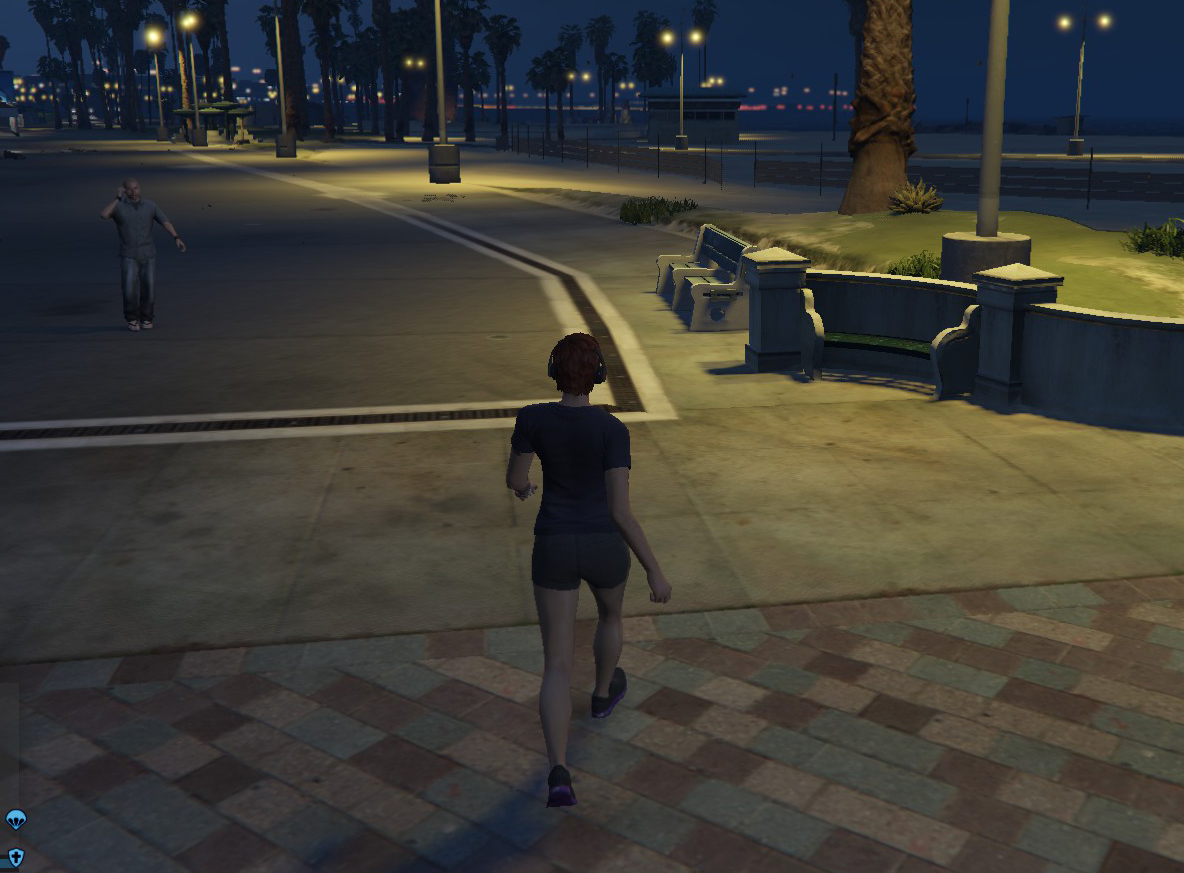
\includegraphics[width=\textwidth]{ExternalMaterial/GTA}
   \caption{A typical third-person view in the game \emph{Grand Theft Auto: IV}. \label{fig:GTAIV}}
\end{figure}

\begin{figure}
   \centering
   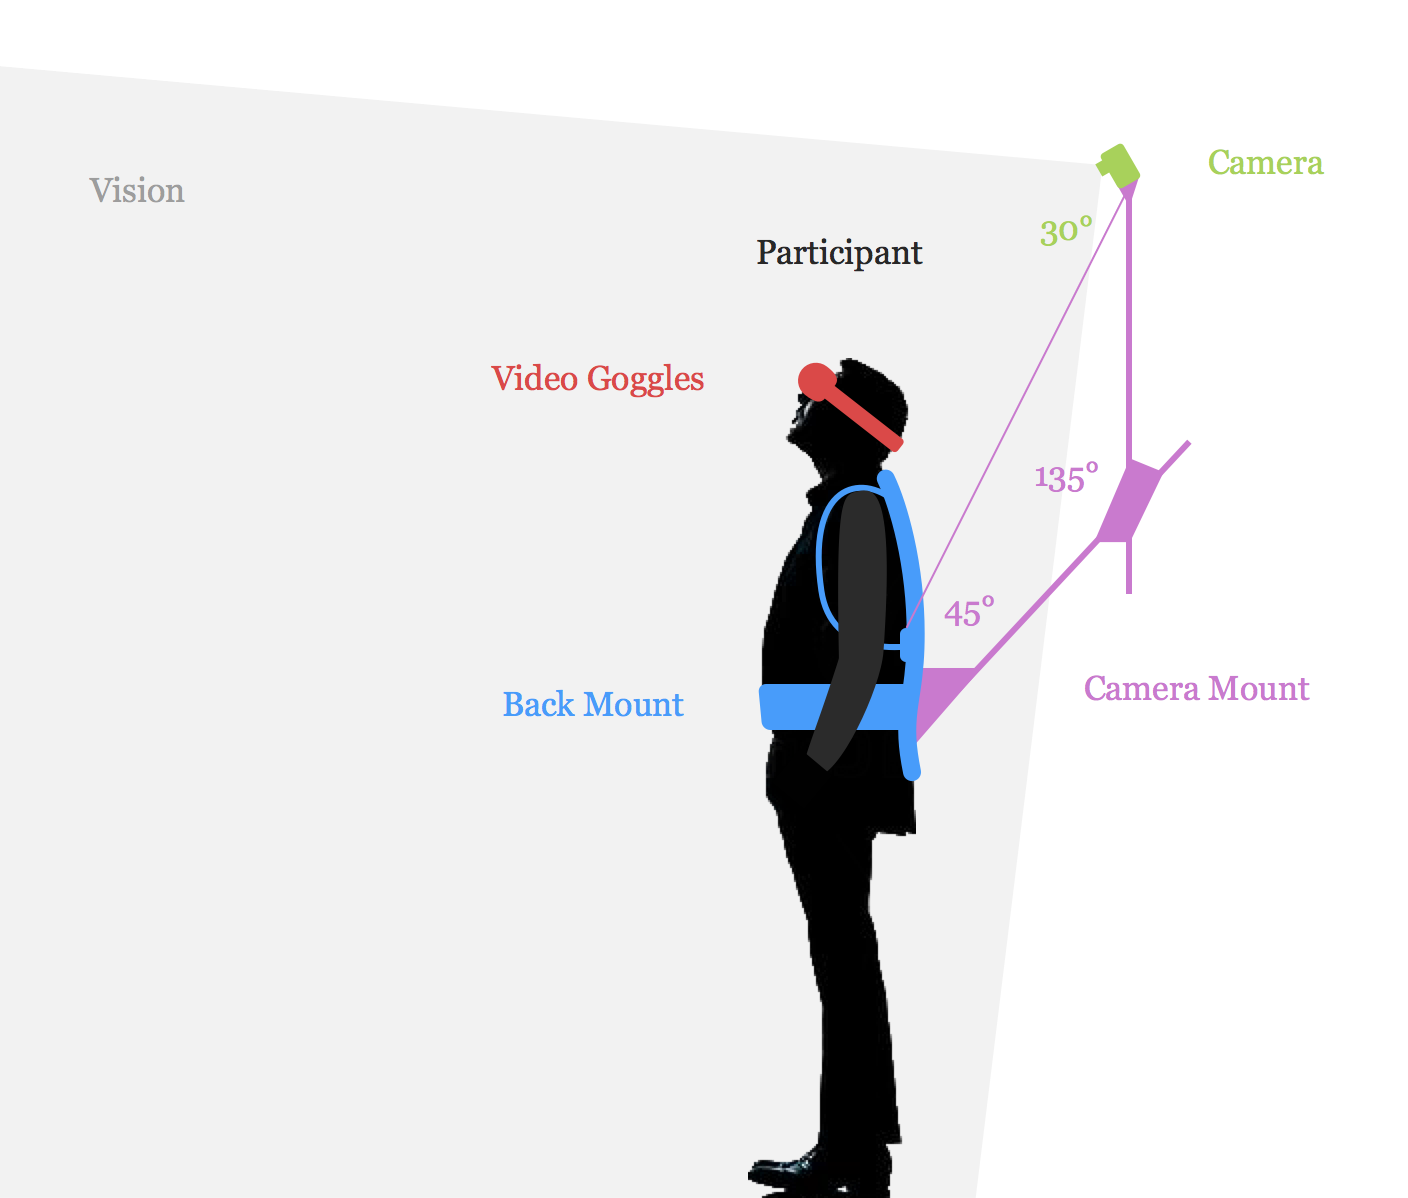
\includegraphics[width=0.5\textwidth]{ExternalMaterial/Rig}
   \caption{A detailed overview of different parts of the rig. \label{fig:RigDesign}}
\end{figure}










% 8888888b.  8888888888 .d8888b.  888     888 888    88888888888 
% 888   Y88b 888       d88P  Y88b 888     888 888        888     
% 888    888 888       Y88b.      888     888 888        888     
% 888   d88P 8888888    "Y888b.   888     888 888        888     
% 8888888P"  888           "Y88b. 888     888 888        888     
% 888 T88b   888             "888 888     888 888        888     
% 888  T88b  888       Y88b  d88P Y88b. .d88P 888        888     
% 888   T88b 8888888888 "Y8888P"   "Y88888P"  88888888   888

\section{Results}
This section will cover the results from the tests that where done and;
\begin{itemize}
	\item The results from the tests
	\item Diagrams comparing the results
	\item Results of earlier work
	\item Compare the performance between the different groups
\end{itemize}











% 8888888b. 8888888 .d8888b.   .d8888b.  888     888  .d8888b.   .d8888b.  
% 888  "Y88b  888  d88P  Y88b d88P  Y88b 888     888 d88P  Y88b d88P  Y88b 
% 888    888  888  Y88b.      888    888 888     888 Y88b.      Y88b.      
% 888    888  888   "Y888b.   888        888     888  "Y888b.    "Y888b.   
% 888    888  888      "Y88b. 888        888     888     "Y88b.     "Y88b. 
% 888    888  888        "888 888    888 888     888       "888       "888 
% 888  .d88P  888  Y88b  d88P Y88b  d88P Y88b. .d88P Y88b  d88P Y88b  d88P 
% 8888888P" 8888888 "Y8888P"   "Y8888P"   "Y88888P"   "Y8888P"   "Y8888P"  

\section{Discussion}
A general discussion about the study such as:
\begin{itemize}
	\item What part/conclusion in my study could be biast/not reliable
	\item What does my results mean?
	\item Earlier work, how do they compare to my work and what does that mean?
	\item References to earlier work such as~\cite{schmierbach2011exploring}
\end{itemize}



\subsection{Limitations and Drawbacks}
Due to the time and budget limit there are several ways to improve upon my study, ways of doing this might include:
\begin{itemize}
	\item Building a more rigid rig.
	\item Using a more comprehensive camera mounted on a stabilized gimbal.
	\item Using more sophisticated video goggles, su. Det är as the Oculus Rift.
\end{itemize}




\subsection{Conclusion}
As a finish, and a complement to the abstract, the conclusion should contain:
\begin{itemize}
	\item What to take out from the study
	\item How this study can be made more in-depth
	\item Future work
\end{itemize}





%\nocite{*}
\bibliographystyle{splncs}
% \bibliographystyle{plain-annote}

\bibliography{Bibliography}

\newpage
\appendix

\section{Appendix}

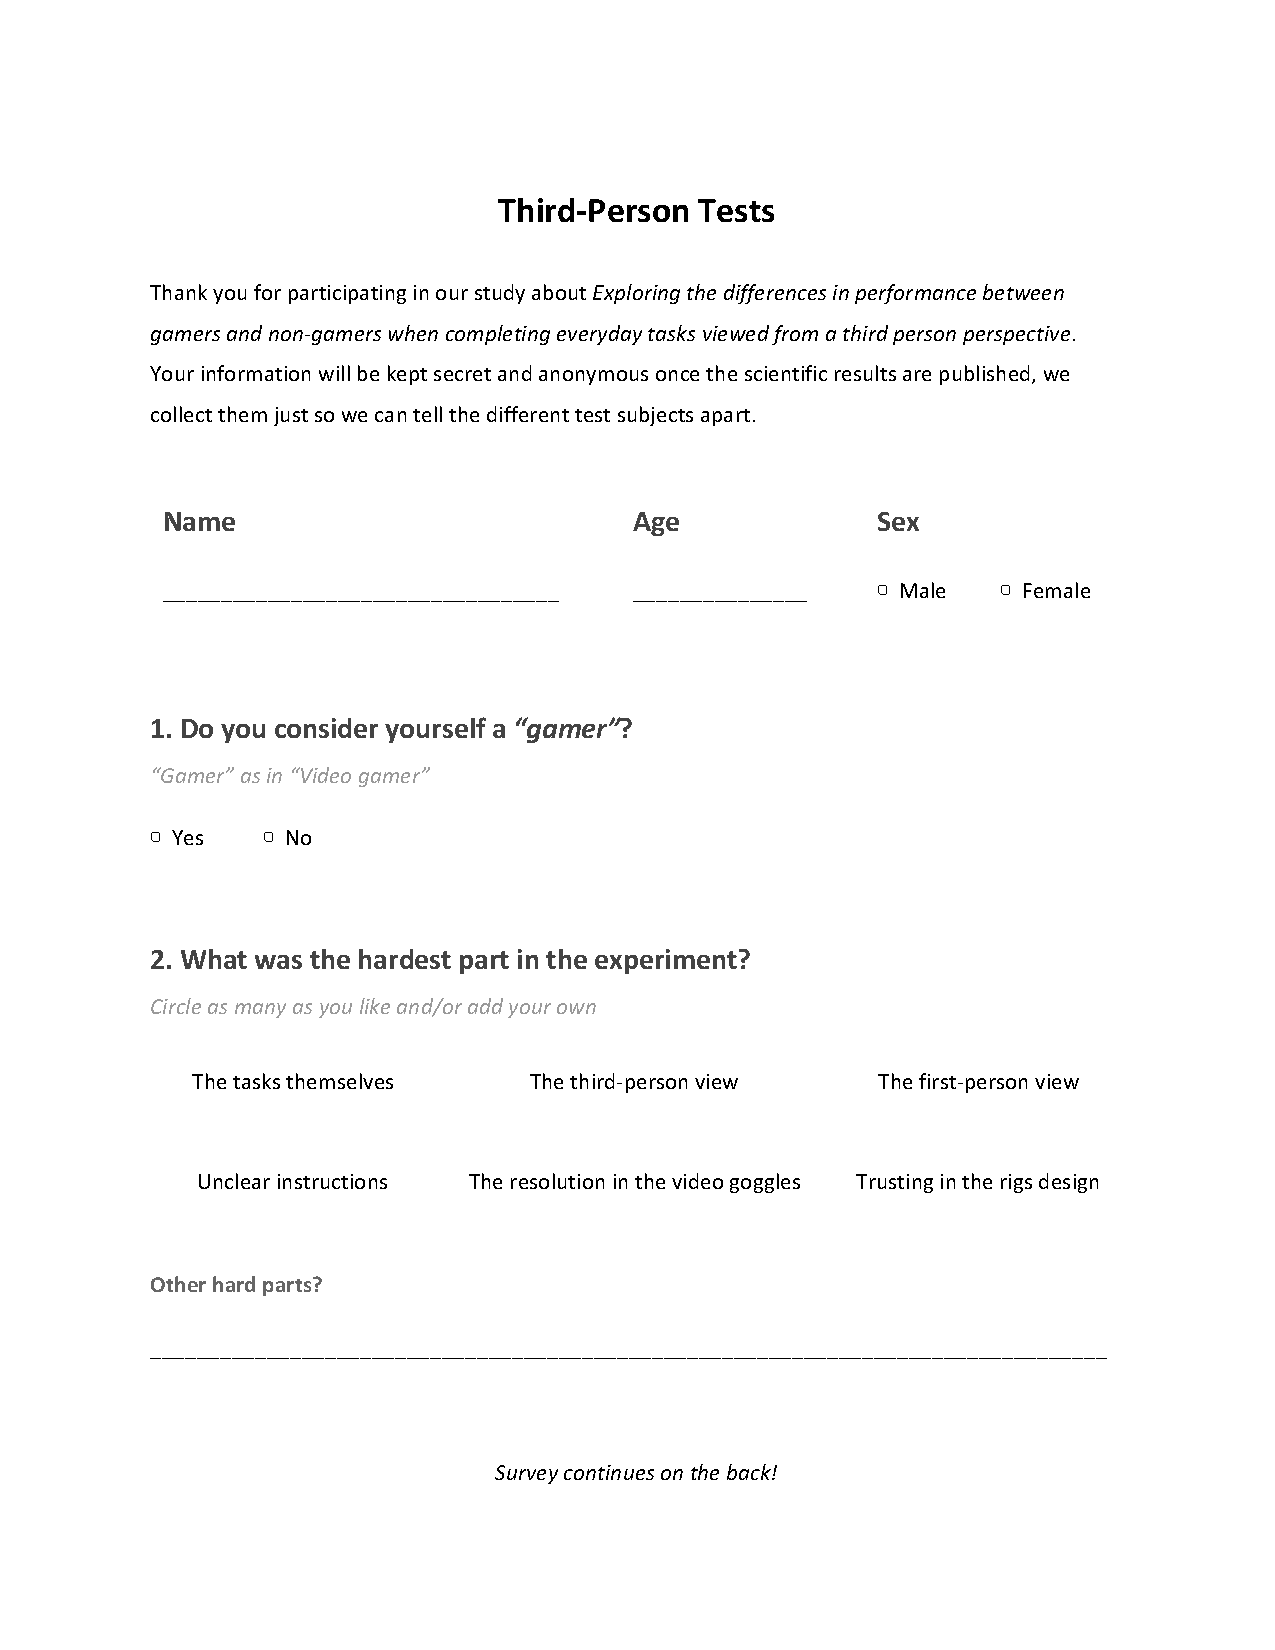
\includepdf[pages={1-2}]{ExternalMaterial/Survey.pdf}


\end{document}